\begin{center}

  \begin{tabular}{rp{16cm}lp{20cm}}%{rl}

  % after \\: \hline or \cline{col1-col2} \cline{col3-col4} ...

  论文地址:& \href{https://ieeexplore.ieee.org/stamp/stamp.jsp?tp=\&arnumber=9046288}{https://ieeexplore.ieee.org/stamp/stamp.jsp?tp=\&arnumber=9046288} \\
  来源:& IEEE Transactions on Neural Networks and Learning Systems, 2020 \\
  作者:& Zonghan Wu, Shirui Pan et.al \\

  %源码:& \href{xxx}{xxx} \\

%  slides:& \href{http://yunshengb.com/wp-content/uploads/2017/03/nips_2018_r2l_workshop_talk.pdf}{{\footnotesize Convolutional Set Matching for Graph Similarity}}\\

  关键词:& \textbf{Deep Learning, graph neural networks, graph convolutional networks, graph representation learning, graph autoencoders} \\

  写于:& \date{2020-12-27}

  \end{tabular}

\end{center}

该论文\cite{9046288}对今年来图神经网络的发展和应用进行了全面的总结,包括对最近的GNNs进行分类、GNNs在不同领域内的应用、开源的代码和基准数据集、GNNs的模型评估以及GNN未来可能的发展方向。

\paragraph{GNNs分类}
该论文将GNNs分为四大类:recurrent gnns RecGNNs)、convolutional gnns(ConvGNNs)、graph autoencoders(GAEs)、spatial-temporal gnns(STGNNs)。

\subparagraph{RecGNNs}
大多是GNNs较为早期的工作,目的是通过循环的神经结构来学习结点/图的表征,结点间一轮一轮地交换信息就相当于循环地过程。\cite{li2015gated}就是其中的一种。RecGNN的结点表征更新如下:
$$
\boldsymbol{h}^{(t)}_v = \sum_{u \in N(v)} f(\boldsymbol{X}_v, \boldsymbol{X}^{\boldsymbol{e}}_{(v,u)}, \boldsymbol{h}^{(t-1)}_u)
$$
其中$f$是recurrent function,该函数应该是一个压缩映射(可以用NN来实现),能够将输入映射到一个更紧凑的空间中。本质上,RecGNNs是基于信息传播的模型的,通过一轮轮的传播来更新表征。

\subparagraph{ConvGNNs}
现在最常见的GNNs --- 图卷积神经网络。ConvGNNs和RecGNNs很像,但是有一个很明显的区别 --- ConvGNNs通过不同的层来完成结点之间信息的交换,且层所代表的映射可以不是压缩映射,且ConvGNNs的层一般都是不一样的,而RecGNNs中的$f$通常都是同一个函数。二者的对比如Fig.\ref{fig:recgnns_convgnns}所示。
\begin{figure}[h]
	\centering
	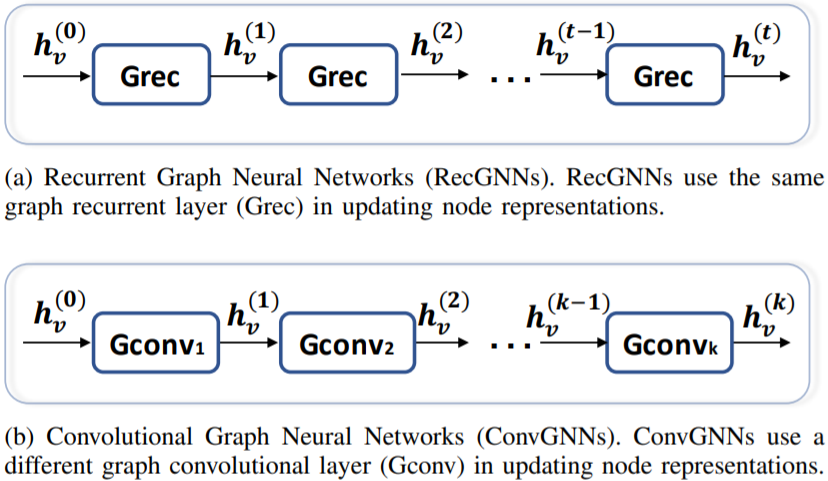
\includegraphics[width=.8\textwidth]{pics/recgnns_convgnns.png}
	\caption{RecGNNs v.s. ConvGNNs}
	\label{fig:recgnns_convgnns}
\end{figure}

在这四种GNNs中,ConvGNNs算是发展得最迅猛、相关工作最多的一类了。ConvGNNs又可以分为两类:Spectral-based ConvGNNs和Spatial-based ConvGNNs。

\textbf{Spectral-based}的方法从图信号处理的角度定义了图卷积。Spectral-based默认graph是无向的,spectral下的图卷积需要对图的Laplacian矩阵进行谱分解$\mathbf{L}=\mathbf{U} \Lambda \mathbf{U}^{T}$,对graph signal进行卷积需要进行\textit{graph Fourier transform},即$\mathscr{F}(\mathbf{x})=\mathbf{U}^{T} \mathbf{x}$,其中$\boldsymbol{x}$为输入的graph signal。图傅里叶变换能够将graph signal变换到由$\boldsymbol{U}$定义的正交空间中。那么给定一个filter(和图像处理领域的滤波器很像)$\boldsymbol{g}$,那么对一个graph signal的卷积定义如下:
$$
\begin{aligned}
	\mathbf{x} *_{G} \mathbf{g} &=\mathscr{F}^{-1}(\mathscr{F}(\mathbf{x}) \odot \mathscr{F}(\mathbf{g})) \\
	&=\mathbf{U}\left(\mathbf{U}^{T} \mathbf{x} \odot \mathbf{U}^{T} \mathbf{g}\right)
\end{aligned}
$$
那么Spectral CNN的定义如下,其中$\Theta_{i, j}^{(k)}$是需要学习的滤波器:
$$
\mathbf{H}_{:, j}^{(k)}=\sigma\left(\sum_{i=1}^{f_{k-1}} \mathbf{U} \Theta_{i, j}^{(k)} \mathbf{U}^{T} \mathbf{H}_{:, i}^{(k-1)}\right) \quad\left(j=1,2, \cdots, f_{k}\right)
$$
spectral-based的图卷积有很坚实的数学基础,但也存在一些局限性:
\begin{itemize}
	\item 不同的结点排列会产生不同的谱分解 --- 不是结点排列无关的
	\item 学习到的滤波器是领域相关的 --- 难以应用到其他领域
	\item 矩阵分解计算复杂 --- 难以应用到large scale graph上
\end{itemize}

\textbf{Spatial-based}即空域的图卷积,是目前的主流。空域的图卷积与图像中的CNN很像。过程:将邻居结点的信息汇聚后,再通过某个函数将结点自身的信息与汇聚后的邻居信息结合起来,与spectral-based的方法相比更直观。在空域卷积的基础上还诞生了图注意力网络 Graph Attention Network。与基础的空域卷积相比,结点与其邻居结点间的权重改由注意力替代。二者的比较如Fig.\ref{fig:gcn_gat}所示:
\begin{figure}[h]
	\centering
	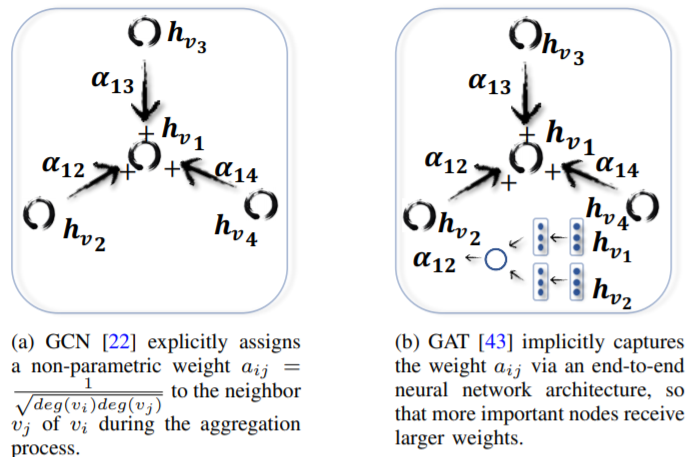
\includegraphics[width=.8\textwidth]{pics/gcn_gat.png}
	\caption{Difference between GCN and GAT}
	\label{fig:gcn_gat}
\end{figure}

除了GAT还出现了与图像领域中类似的操作,如Graph Pooling,功能也与图像领域的池化操作类似 --- 降低图的规模/从结点表征矩阵产生图表征(Readout)。

\subparagraph{GAEs}
图自编码器 --- encoder将graph的结点映射到隐空间中,decoder将隐空间中的图还原/重建。GAEs可以用来学习结点的表征以及生成图。一个现有的GAEs的一个统计表如Fig.\ref{fig:gaes}所示。
\begin{figure}[h]
	\centering
	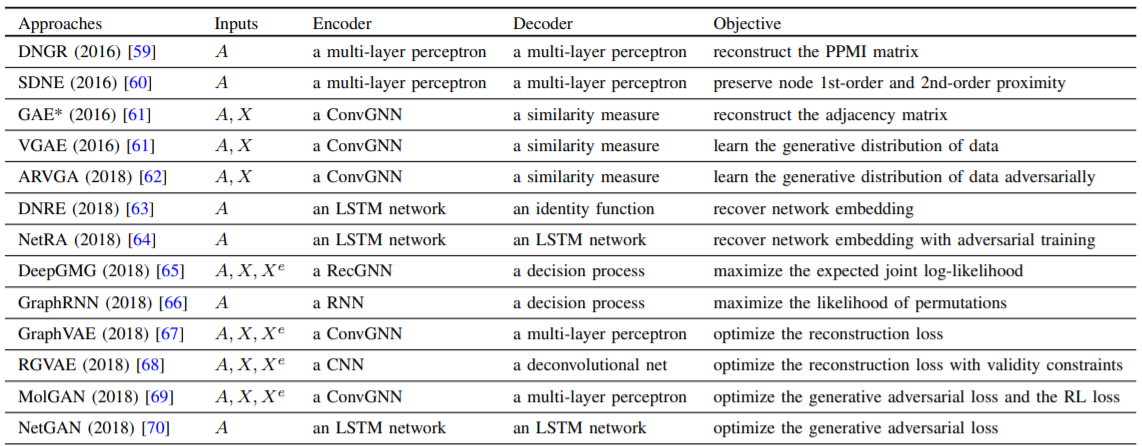
\includegraphics[width=.8\textwidth]{pics/gaes.png}
	\caption{ Main characteristics of selected GAEs}
	\label{fig:gaes}
\end{figure}
使用GAEs来生成图可以分为两类:Sequential --- 逐步地增减结点/边,Global --- 一次性生成整个graph。

\subparagraph{STGNNs}
时空地图神经网络,这种GNNs主要用在dynamic graphs上 --- 捕捉时间序列地特征/分布,序列与graph的联合/边缘分布,graph在时间、空间上的关系。STGNNs的任务可以是预测预测结点的值/标签或者graph的便签 --- 当然是结合时间的。常见的应用场景包括流式的图数据、交通数据(如交通中的流量、速度等数据)等。STGNNs目前主要由两个发展方向:RNN-based和CNN-based。

RNN-based方法会单独处理每一个时刻的图数据,并作为输入流入下一个时刻的处理步骤。有些方法会将结点和边分开来处理 --- 分别输入RNN-based处理单元中。CNN-based方法以非循环的方式来处理,RNN-based和CNN-based有点像RecGNNs和ConvGNNs,CNN-based方法通过堆叠多层网络来处理dynamic graph。

\paragraph{GNNs应用}
\subparagraph{Computer Vision}
包括场景图生成、点云数据分类、动作识别。在场景图中,GNNs可以帮助识别对象之间的语义关系,与之相反的是场景图的生成,将自然语言描述的场景生成为场景图。

\subparagraph{Natural Language Processing}
GNNs可以借助文本中句子/词之间的关系来对文本进行分类,除此之外,在NLP领域还有很多自然的grpah-like数据,如语法依存树。同时也可以基于语义图(semantic graph)来生成文本或者反过来。

\subparagraph{Traffic}
例如动态预测道路的可行驶速度、流量等,这通常与STGNNs联系起来。通常将交通网络看作时空图,其中的结点为安装在路上的传感器、边表示传感器之间的距离,这样每个结点在一定的时间区间内都有自己的流速。

\subparagraph{Recommender system}
Graph-based的推荐系统通常将用户、商品视作结点,通过利用结点之间的关系以及与相关的信息融合起来进行推荐。推荐系统的一个关键点:针对一个用户,给出每个商品对其的重要性排序/分数,这也可以转化为一个链接预测问题 --- 预测用户和商品之间的链接。

\subparagraph{Chemistry}
在生物/化学/生物信息领域,通常利用GNNs来研究分子/化合物/药物的结构 --- 这些东西也天然地具有graph结构。

\subparagraph{Others}
除了上述的几个主要的应用领域,还存在一些比较小众/还未广泛研究的领域,例如程序验证、程序推理、社会影响力预测、对抗攻击防御、异常检测、脑网络研究等。

\paragraph{GNNs模型评估}
在GNNs中有几个主要的任务:结点分类、图分类、链接预测(我自己补充的)。

\paragraph{常用数据集}
常见的数据如Fig.\ref{fig:benchmark}所示.
\begin{figure}[h]
	\centering
	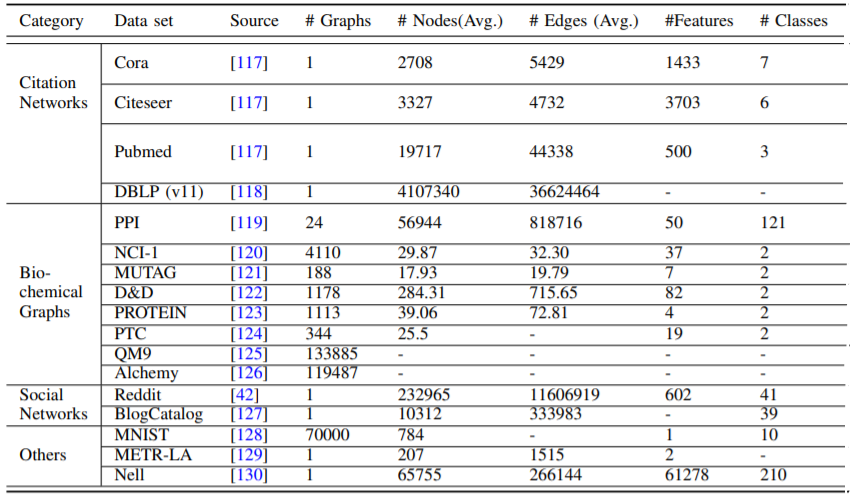
\includegraphics[width=.8\textwidth]{pics/benchmark_datasets.png}
	\caption{Summary of benchmark datasets}
	\label{fig:benchmark}
\end{figure}

\paragraph{未来发展方向}
\subparagraph{Model Depth}
就目前的情况来看,GNNs的模型都比较浅,与CNN模型动则数十层的模型相比,GNNs的模型层数都比较少。当GNN中层数较多时,基本上每个结点的信息都已经被传播到了图中其余的结点 --- 通常图的最短路径会在6跳左右/六度分隔,这也导致当层数一多,图中结点的表征就会趋于一致,这反而使得结点的表征不具有区分性。\tbc{red}{如何加深GNNs或者什么情况下需要深度的GNNs是一个很值得研究的问题}。

\subparagraph{Scalability trade-off}
伸缩性权衡。GNNs的可伸缩性是以破坏图的完整性为代价的。在现有的GNNs中,通常会有ZPooling和Coarsening操作来降低节点特征的维度或者图的规模,但是这些操作都或多或少的丢失了一部分信息。如何设计一个破坏图数据完整性的GNN或者如何权衡完整性和可行性是一个很值得研究的问题。

\subparagraph{Hetergenity}
GNNs在异质图数据上的应用。目前大多数的GNNs处理的是同质的图数据 --- 结点都为同一类型或者只有一种类型,边也只有一种类型,但是还有很多数据是异质的 --- 结点/边的类型是多样的,以及结点/边的输入形式都是不一样的,例如结点/边为文本/图像等,这可以视作现在的多模态融合问题,相当于以GNNs来进行多模态数据融合。

\subparagraph{Dynamicity}
虽然已经有STGNNs来处理随时间变化的图数据,但是大部分都没有dynamic spatioal relations(\textbf{这里我不太理解})。不过确实需要设计更好的处理动态的图数据、流式的图数据(\tbc{red}{流式的数据处理是一个很有意思的问题})。

这篇综述是2019年发表的,虽然在2020年已经出现了很多新的关于GNNs的工作,一些工作也与文中谈的一些问题重叠了,但是这篇综述依然是一片很全面、详细的对GNNs今年来的工作的总结,提出的问题也很具有参考性,是一篇非常棒的综述!




